\chapter{Desenvolvimento da aplicação}
O desenvolvimento da aplicação SheSafe fundamentou-se em princípios sólidos de engenharia de software, adotando arquiteturas e padrões consolidados que garantem manutenibilidade, escalabilidade e testabilidade do código. Este capítulo apresenta as decisões arquiteturais, tecnologias empregadas e a estrutura organizacional do projeto, demonstrando como a aplicação de conceitos teóricos de desenvolvimento de software materializou-se em uma solução tecnológica funcional.

\section{Arquitetura e Padrões de Projeto}
\subsection{Arquitetura Limpa (Clean Architecture)}
A aplicação SheSafe foi estruturada seguindo os princípios da Arquitetura Limpa proposta por Robert C. Martin \cite{martin2017clean}, organizando o código em camadas concêntricas com dependências unidirecionais que fluem das camadas externas para as camadas internas. Esta abordagem arquitetural visa maximizar a independência de frameworks, interfaces de usuário, bancos de dados e agentes externos, promovendo um design que facilita testes e manutenção.
\begin{figure}[H]
	\centering
	 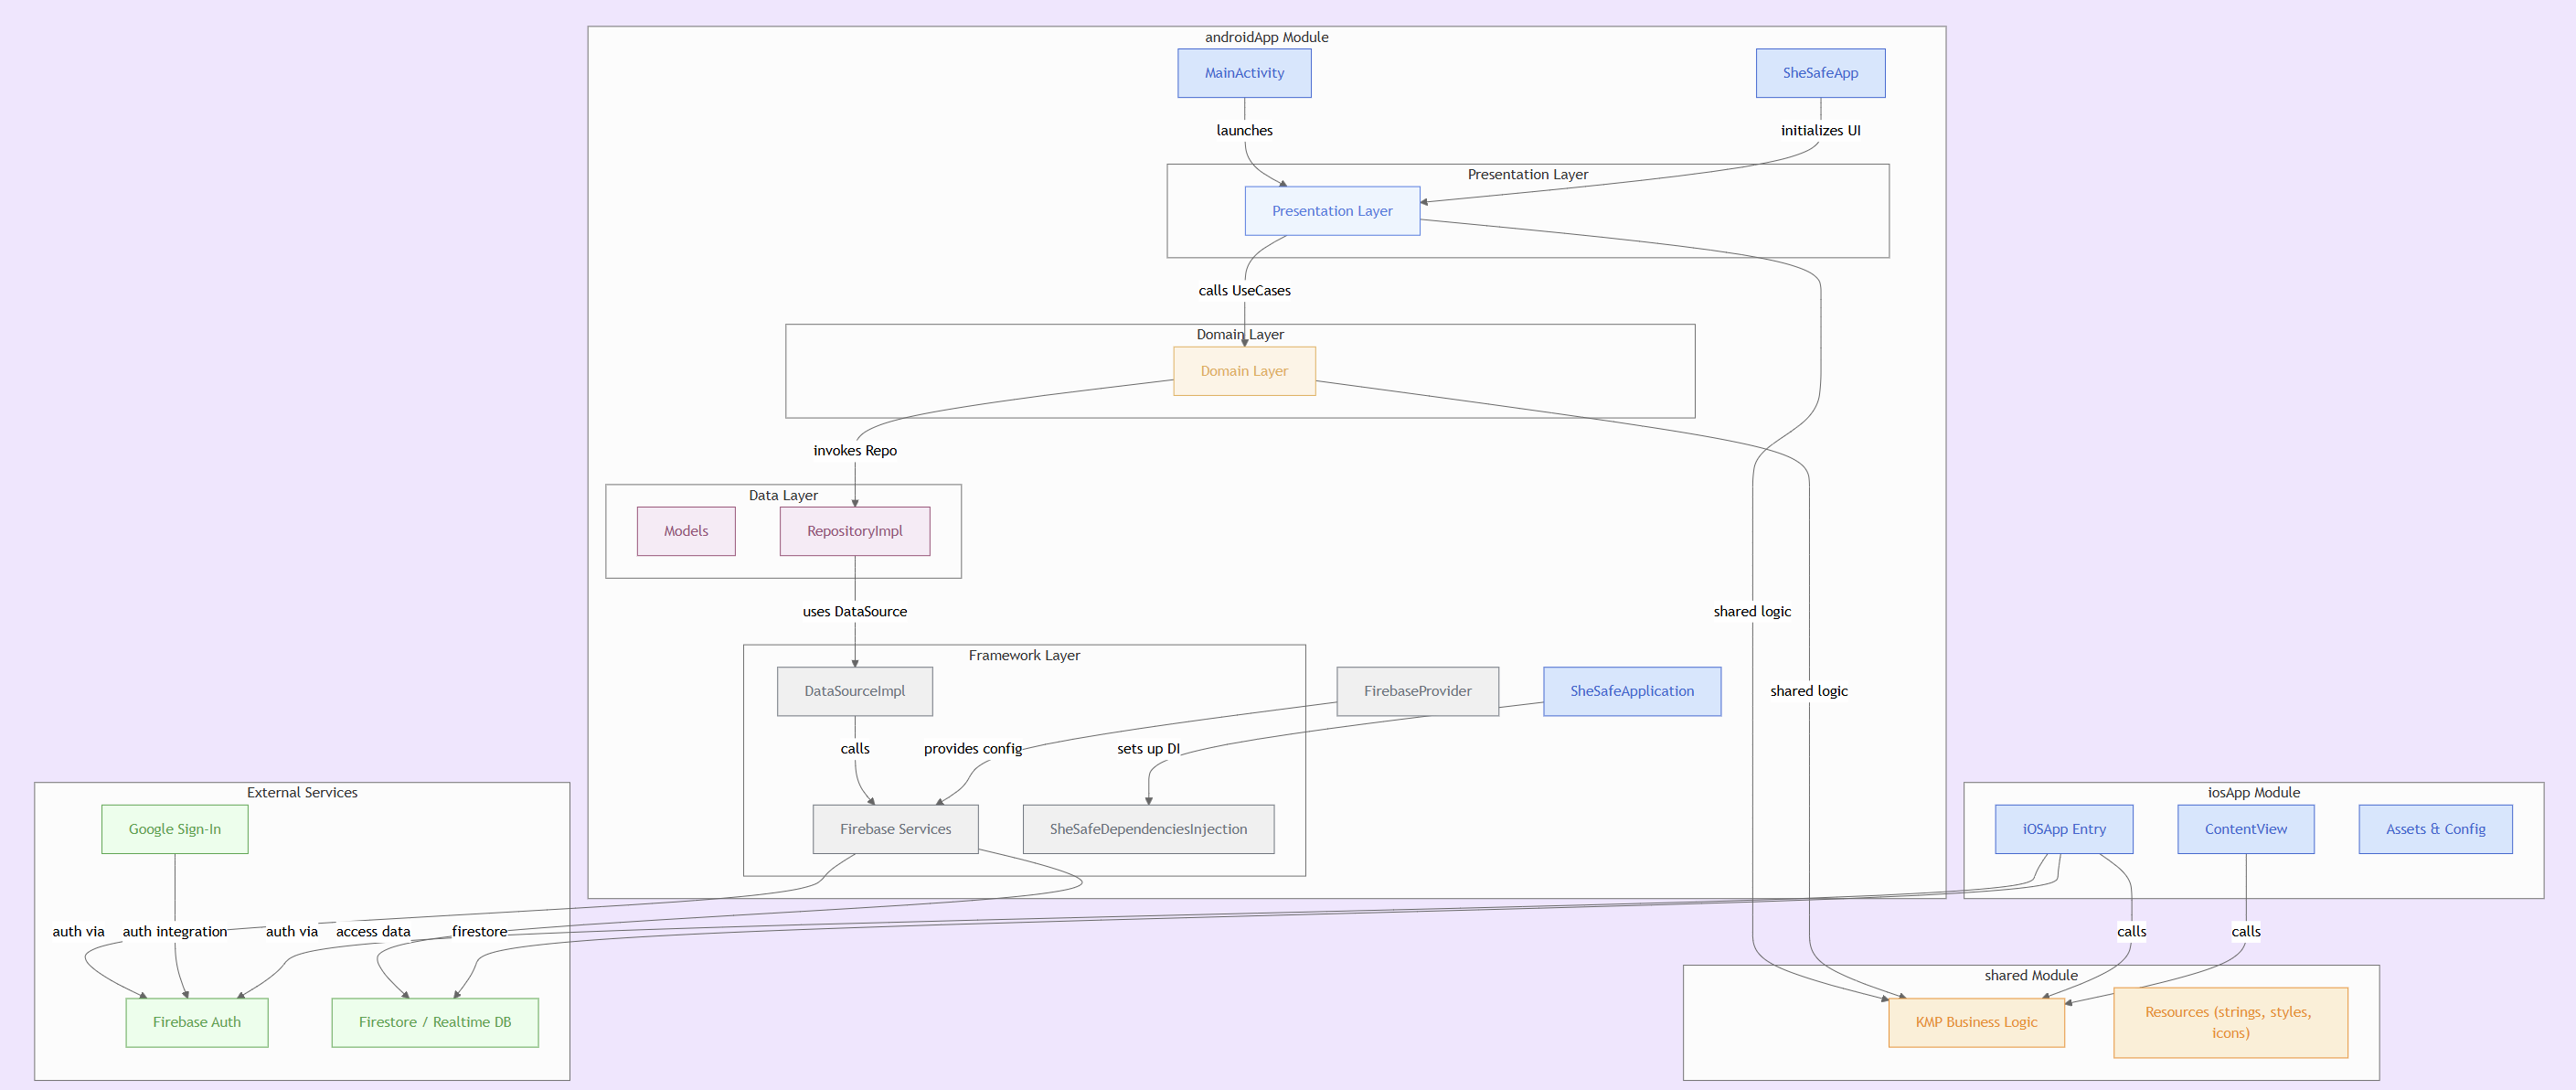
\includegraphics[width=0.8\linewidth]{images/shesafe/shesafe-architecture.png}\\
	\caption{Diagrama ilustrativo das camadas da Clean Architecture aplicada ao SheSafe}
	\label{fig:clean_architecture}
	\legend{Fonte: Próprio Autor}
\end{figure}
A estrutura de camadas implementada no projeto pode ser observada na organização dos pacotes dentro do módulo \texttt{androidApp}, conforme ilustrado na estrutura de diretórios do projeto:
\begin{figure}[H]
	\centering
	 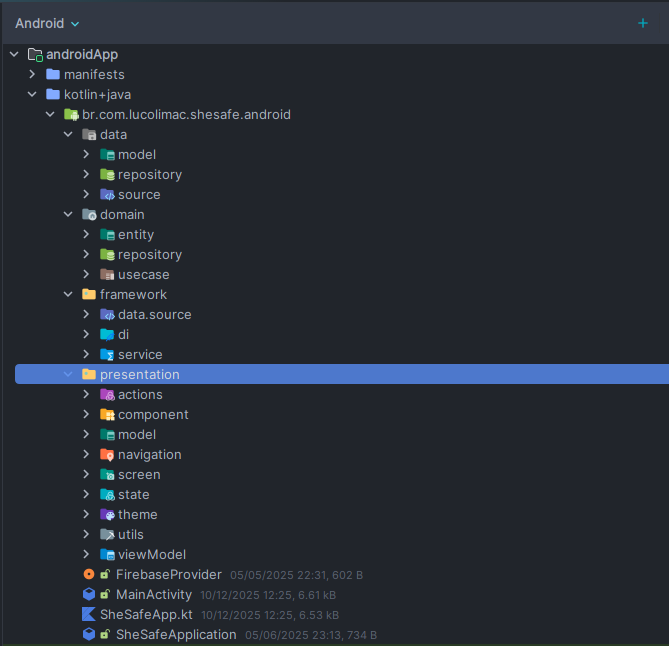
\includegraphics[width=0.8\linewidth]{images/shesafe/screenshot-clean-architecture-shesafe.png}\\
	\caption{Screenshot da estrutura de pastas do módulo androidApp mostrando os pacotes domain, data, framework e presentation}
	\label{fig:estrutura_pastas_androidapp}
\end{figure}
\subsubsection{Camada de Domínio (Domain Layer)}
A camada de domínio representa o núcleo da aplicação, contendo as regras de negócio e entidades fundamentais do sistema. Esta camada é completamente independente de frameworks e tecnologias específicas, garantindo que a lógica de negócio permaneça isolada de detalhes de implementação. No projeto SheSafe, a camada de domínio está organizada no pacote \path{br.com.lucolimac.shesafe.android.domain} e compreende três subpacotes principais:

O subpacote \texttt{entity} contém as classes que representam os conceitos centrais do domínio da aplicação. As entidades \texttt{SecureContact} e \texttt{HelpRequest} encapsulam respectivamente as informações de contatos seguros cadastrados pelo usuário e os registros de pedidos de ajuda enviados. Estas entidades são classes de dados (\textit{data classes}) em Kotlin que implementam a interface \texttt{Parcelable}, permitindo sua serialização para passagem entre componentes Android. A entidade \texttt{HelpRequest} inclui lógica de domínio para geração de links do Google Maps baseados nas coordenadas de geolocalização, exemplificando como regras de negócio podem ser encapsuladas nas próprias entidades.

O subpacote \texttt{repository} define interfaces que especificam contratos para acesso a dados, sem se preocupar com os detalhes de implementação do armazenamento. As interfaces \texttt{SecureContactRepository}, \texttt{HelpRequestRepository}, \texttt{SettingsRepository}, \texttt{AuthRepository} e \texttt{HelpMessageRepository} declaram métodos para operações de leitura e escrita de dados, todas com modificador \texttt{suspend} indicando que são funções assíncronas executadas em corrotinas Kotlin. Esta abstração permite que a camada de domínio permaneça independente de decisões sobre qual tecnologia de persistência será utilizada, seja Firebase Firestore, banco de dados local ou qualquer outra solução.

O subpacote \texttt{usecase} implementa casos de uso da aplicação, representando as operações específicas que o sistema pode realizar. Cada caso de uso é definido por uma interface (como \texttt{SecureContactUseCase}, \texttt{HelpRequestUseCase}, \texttt{SettingsUseCase}, \texttt{AuthUseCase} e \texttt{HelpMessageUseCase}) e sua respectiva implementação (sufixo \texttt{Impl}). Os casos de uso orquestram a interação com repositórios e aplicam regras de negócio específicas, retornando dados através de \texttt{Flow}, uma construção de programação reativa do Kotlin que permite emissão assíncrona de valores. A implementação dos casos de uso utiliza \texttt{CoroutineDispatcher} configurado para \texttt{Dispatchers.IO}, garantindo que operações de I/O sejam executadas em threads apropriadas.

\subsubsection{Camada de Dados (Data Layer)}
A camada de dados atua como intermediária entre a camada de domínio e as fontes de dados externas, implementando os contratos definidos pelos repositórios e abstraindo os detalhes de acesso aos dados. Esta camada está organizada no pacote \path{br.com.lucolimac.shesafe.android.data} e subdivide-se em três componentes principais.

O subpacote \texttt{model} contém classes de modelo de dados (DTOs -- \textit{Data Transfer Objects}) que representam a estrutura dos dados conforme armazenados no Firebase Firestore. As classes \texttt{SecureContactModel} e \texttt{HelpRequestModel} incluem construtores vazios necessários para desserialização do Firestore, anotações \texttt{@SerializedName} do Gson para mapeamento de campos JSON, e métodos de conversão bidirecionais (\texttt{toEntity()} e \texttt{fromEntity()}) que transformam modelos de dados em entidades de domínio e vice-versa. Esta separação entre modelos de dados e entidades de domínio permite que mudanças na estrutura de armazenamento não afetem a lógica de negócio.

O subpacote \texttt{repository} fornece implementações concretas das interfaces de repositório definidas na camada de domínio. Classes como \texttt{SecureContactRepositoryImpl}, \texttt{HelpRequestRepositoryImpl}, \texttt{SettingsRepositoryImpl}, \texttt{AuthRepositoryImpl} e \texttt{HelpMessageRepositoryImpl} delegam operações para as respectivas fontes de dados, realizando conversões necessárias entre modelos e entidades. Estas implementações utilizam injeção de dependência para receber instâncias de \texttt{DataSource}, promovendo baixo acoplamento e facilitando testes unitários.

O subpacote \texttt{source} define interfaces abstratas de fontes de dados (\texttt{SecureContactDataSource}, \texttt{HelpRequestDataSource}, \texttt{SettingsDataSource}, \texttt{AuthDataSource} e \texttt{HelpMessageDataSource}) que especificam operações de acesso aos dados sem revelar detalhes de implementação específicos. Esta abstração adicional permite que diferentes implementações de armazenamento (Firebase, banco de dados local, API REST) sejam intercambiadas sem afetar as camadas superiores.

\subsubsection{Camada de Framework (Framework Layer)}
A camada de framework contém as implementações concretas que interagem diretamente com tecnologias e frameworks específicos, neste caso, o Firebase. Localizada no pacote \path{br.com.lucolimac.shesafe.android.framework}, esta camada materializa as abstrações definidas nas camadas superiores através de componentes específicos de infraestrutura.

O subpacote \texttt{service} contém interfaces de serviço e suas implementações Firebase. As interfaces \texttt{SecureContactService}, \texttt{HelpRequestService}, \texttt{SettingsService}, \texttt{AuthService} e \texttt{HelpMessageService} definem contratos para operações específicas, enquanto suas implementações (sufixo \texttt{FirebaseService}) realizam operações reais no Firestore e Firebase Authentication. Por exemplo, \texttt{SecureContactFirebaseService} utiliza a instância de \texttt{FirebaseFirestore} para acessar coleções específicas do usuário autenticado, implementando operações CRUD através da API assíncrona do Firebase com suporte a corrotinas Kotlin (\texttt{await()}).

O subpacote \texttt{data.source} fornece implementações concretas das interfaces \texttt{DataSource}, delegando operações para os serviços Firebase correspondentes. Classes como \texttt{SecureSecureContactDataSourceImpl}, \texttt{HelpRequestDataSourceImpl}, \texttt{SettingsDataSourceImpl}, \texttt{AuthDataSourceImpl} e \texttt{HelpMessageDataSourceImpl} tratam exceções e convertem resultados conforme necessário, atuando como adaptadores entre as abstrações da camada de dados e os serviços concretos do framework.

O subpacote \texttt{di} (\textit{Dependency Injection}) contém a configuração de injeção de dependências utilizando o framework Koin. O objeto \texttt{SheSafeDependenciesInjection} define o módulo Koin que registra todas as dependências do projeto, estabelecendo como instâncias de serviços, fontes de dados, repositórios, casos de uso e ViewModels devem ser criadas e injetadas. Esta configuração centralizada facilita a gestão de dependências e promove testabilidade através da possibilidade de substituir implementações reais por mocks durante testes.
\section{Avaliação com usuário}
A avaliação com usuário constitui-se como um paradigma metodológico fundamental no campo da Interação Humano-Computador (IHC), caracterizado pela participação direta de usuários reais no processo de análise e validação de sistemas interativos \cite{dix2003human}. Esta abordagem fundamenta-se no princípio de que a qualidade de um sistema deve ser mensurada a partir da perspectiva de quem efetivamente o utiliza, considerando suas necessidades, expectativas, limitações cognitivas e contextos de uso específicos \cite{preece2015interaction}.

Diferentemente dos métodos de inspeção realizados por especialistas, a avaliação com usuário oferece insights diretos sobre a experiência real de interação, revelando aspectos que podem não ser identificados através de análises teóricas ou heurísticas \cite{nielsen1994usability}. Esta metodologia permite a observação de comportamentos autênticos, identificação de estratégias de uso não previstas pelos designers, e compreensão das dificuldades reais enfrentadas pelos usuários em contextos naturais de utilização.

\subsection{Avaliação do usuário SheSafe}
As avaliações com usuário da aplicação SheSafe foram conduzidas entre os dias 24 e 28 de setembro de 2025, envolvendo participantes que executaram três tarefas específicas relacionadas às funcionalidades principais do sistema. Os testes foram realizados com a versão debug da aplicação Android, disponibilizada através de um link de download compartilhado.

Em relação ao cumprimento dos objetivos das tarefas, os resultados demonstraram 100\% de taxa de sucesso, com todas as participantes conseguindo completar as três atividades propostas: enviar um pedido de socorro pela primeira vez, cadastrar um novo contato seguro e alterar a mensagem padrão do pedido de ajuda. Não foram registrados erros durante a execução de nenhuma das tarefas, indicando que a interface apresenta boa intuitividade e que os fluxos de interação estão adequadamente projetados para facilitar a conclusão das ações pelos usuários.

Na \autoref{tab:mediadetempo} é possível ver a média de tempo dos testes com os usuários para cada uma das três jornadas analisadas. Ela nos mostra uma performance satisfatória em todas as tarefas avaliadas. Para o envio do primeiro pedido de socorro, os tempos variaram entre 21 e 31 segundos, com média de 25,3 segundos. O cadastro de contatos seguros apresentou tempos mais consistentes, variando entre 13 e 17 segundos (média de 14,3 segundos). A alteração da mensagem padrão foi a tarefa executada mais rapidamente, com tempos entre 11 e 14 segundos (média de 12,3 segundos). Esta progressão temporal sugere que as funcionalidades mais críticas mantêm tempos de resposta adequados para situações de emergência, enquanto as funcionalidades de configuração são executadas de forma ainda mais eficiente.

\begin{table}[htbp]
	\centering
	\caption[Média de tempo de execução]{Média de tempo de execução}
	\label{tab:mediadetempo}
	\begin{tabular}{cc}
		\hline
		\multicolumn{1}{|c|}{Tarefa}                                        & \multicolumn{1}{c|}{Tempo médio}            \\ \hline \hline
		\multicolumn{1}{|c|}{Enviar um pedido de socorro pela primeira vez} & \multicolumn{1}{c|}{0} \\ \hline
		\multicolumn{1}{|c|}{Cadastrar um novo contato seguro}              & \multicolumn{1}{c|}{0} \\ \hline
		\multicolumn{1}{|c|}{Alterar a mensagem padrão do pedido de ajuda}  & \multicolumn{1}{c|}{0} \\ \hline
	\end{tabular}
	\fonte{Próprio Autor}
\end{table}


No que se refere às impressões qualitativas, as avaliadoras expressaram percepções predominantemente positivas sobre diferentes aspectos da aplicação. A navegação foi consistentemente avaliada como adequada por todas as participantes, assim como o design visual e a usabilidade geral do sistema.
\begin{comment}
	Mônica Abreu destacou especificamente que "a interface é muito fácil e simples de aprender a utilizar", enquanto Wannielly Barbosa elogiou a "navegação fluida e sem problema para mudar de tela", caracterizando ainda a iniciativa como "ótima para mulheres".
\end{comment}

Contudo, emergiu um padrão consistente de feedback relacionado à ausência de confirmações explícitas do sistema após a execução de determinadas ações. Algumas das avaliadoras relataram especificamente a "falta de um retorno ao cadastrar o contato", enquanto uma outra observou que "ao alterar mensagem, só vi que alterou quando mudou na tela". Este feedback indica uma oportunidade de melhoria significativa no design de interação, particularmente na implementação de feedback imediato e explícito para ações críticas do usuário.

A convergência deste feedback específico sobre a ausência de confirmações do sistema sugere que esta deficiência pode impactar negativamente a confiança do usuário na aplicação, especialmente em um contexto de uso onde a certeza sobre a execução correta das ações é fundamental para a eficácia do sistema de segurança. A implementação de mensagens de confirmação, notificações toast, ou outros elementos de feedback visual imediato deveria ser considerada como prioridade para futuras iterações do desenvolvimento, visando aumentar a transparência do sistema e a confiança do usuário nas operações realizadas.L